\chapter{MARCO METODOL\'OGICO}

Este capítulo describe el diseño experimental adoptado para alcanzar los objetivos de la
investigación. La exposición sigue el flujo lógico de la ejecución: datos y particionamiento,
arquitecturas evaluadas, protocolo de federación, instrumentación de métricas y procedimiento
de análisis. Toda la información necesaria para replicar los experimentos queda documentada
en esta sección.

% ============================================================
\section{Diseño del Estudio}
% ============================================================

La investigación adoptó un enfoque cuantitativo y experimental. Se manipularon tres variables
independientes —familia arquitectónica, grado de heterogeneidad estadística y algoritmo de
agregación— y se midió su efecto sobre variables dependientes de rendimiento, drift paramétrico
y similitud de representaciones. Las variables intervinientes (inicialización, optimizador,
número de rondas, datos de prueba) se mantuvieron constantes en todos los experimentos.

La dimensión temporal es inherente al diseño: el drift, la convergencia y la evolución de
representaciones se registraron en cada una de las $T = 50$ rondas de comunicación, lo que
permite analizar la dinámica del proceso federado y no únicamente su estado final.

\subsection{Variables del estudio}

\textbf{Variables independientes.}
\begin{itemize}
  \item \textit{Arquitectura del modelo}: EfficientNet-B1 (BatchNorm), EfficientNet-B1
    (GroupNorm-32), EfficientNet-B1 (LayerNorm/GN-1), ViT-Tiny, Vim-Tiny, ViG-Tiny y ResNet-9.
  \item \textit{Nivel de heterogeneidad no-IID}: $\alpha \in \{1000, 1.0, 0.3, 0.1, 0.03\}$,
    controlado mediante la concentración de la distribución de Dirichlet.
  \item \textit{Algoritmo de agregación federada}: FedAvg y FedProx ($\mu = 0.01$).
\end{itemize}

\textbf{Variables dependientes.}
\begin{itemize}
  \item Rendimiento: accuracy global, F1-score macro, precision y recall sobre el test global.
  \item Convergencia: primera ronda en que la accuracy cruza el umbral correspondiente y
    permanece por encima durante cinco rondas consecutivas.
  \item Equidad inter-cliente (\textit{fairness}): brecha de accuracy entre el cliente mejor
    y el peor al final del entrenamiento.
  \item Drift paramétrico: norma $L_2$ normalizada por grupo de capas \{norm, feature, head\}.
  \item Alineación de gradientes: similitud coseno pairwise inter-cliente por grupo de capas.
  \item Drift representacional: Centered Kernel Alignment (CKA) global-vs-cliente y pairwise
    inter-cliente por capa y por ronda.
\end{itemize}

\textbf{Variables intervinientes (controladas).}
Número de clientes $K = 10$, participación completa en cada ronda, $E = 5$ épocas locales,
tamaño de batch $B = 32$, SGD con $\text{lr} = 0.01$, momentum $= 0.9$, weight decay $= 10^{-4}$,
inicialización aleatoria (sin pesos preentrenados), semillas $\{42, 123, 456\}$, y el mismo
conjunto de test global para todos los clientes y modelos.

% ============================================================
\section{Conjuntos de Datos}
% ============================================================

\subsection{Brain Tumor MRI}

El dataset principal fue el Brain Tumor MRI Dataset de Kaggle \cite{msoud_nickparvar_2026},
compuesto por $7\,023$ imágenes de resonancia magnética distribuidas en cuatro clases:
glioma, meningioma, pituitario y no-tumor. La división de entrenamiento y prueba totalizó
5\,712 y 1\,311 imágenes, respectivamente. Todas las imágenes se redimensionaron a
$224 \times 224$ píxeles para compatibilidad con el tokenizador de parches de ViT-Tiny
($16 \times 16$) y para eliminar la resolución de entrada como variable de confusión en la
comparación entre familias. Las imágenes en escala de grises se convirtieron a tres canales
mediante \texttt{transforms.Grayscale(3)}.

El pipeline de preprocesamiento para entrenamiento incluyó volteo horizontal aleatorio
($p = 0.5$), rotación aleatoria ($\pm 15^{\circ}$), perturbación de brillo y contraste
($\pm 0.2$), y normalización con las estadísticas de ImageNet. Para el test, únicamente
se aplicó redimensionamiento y normalización.


\begin{figure}[htbp]
  \centering
  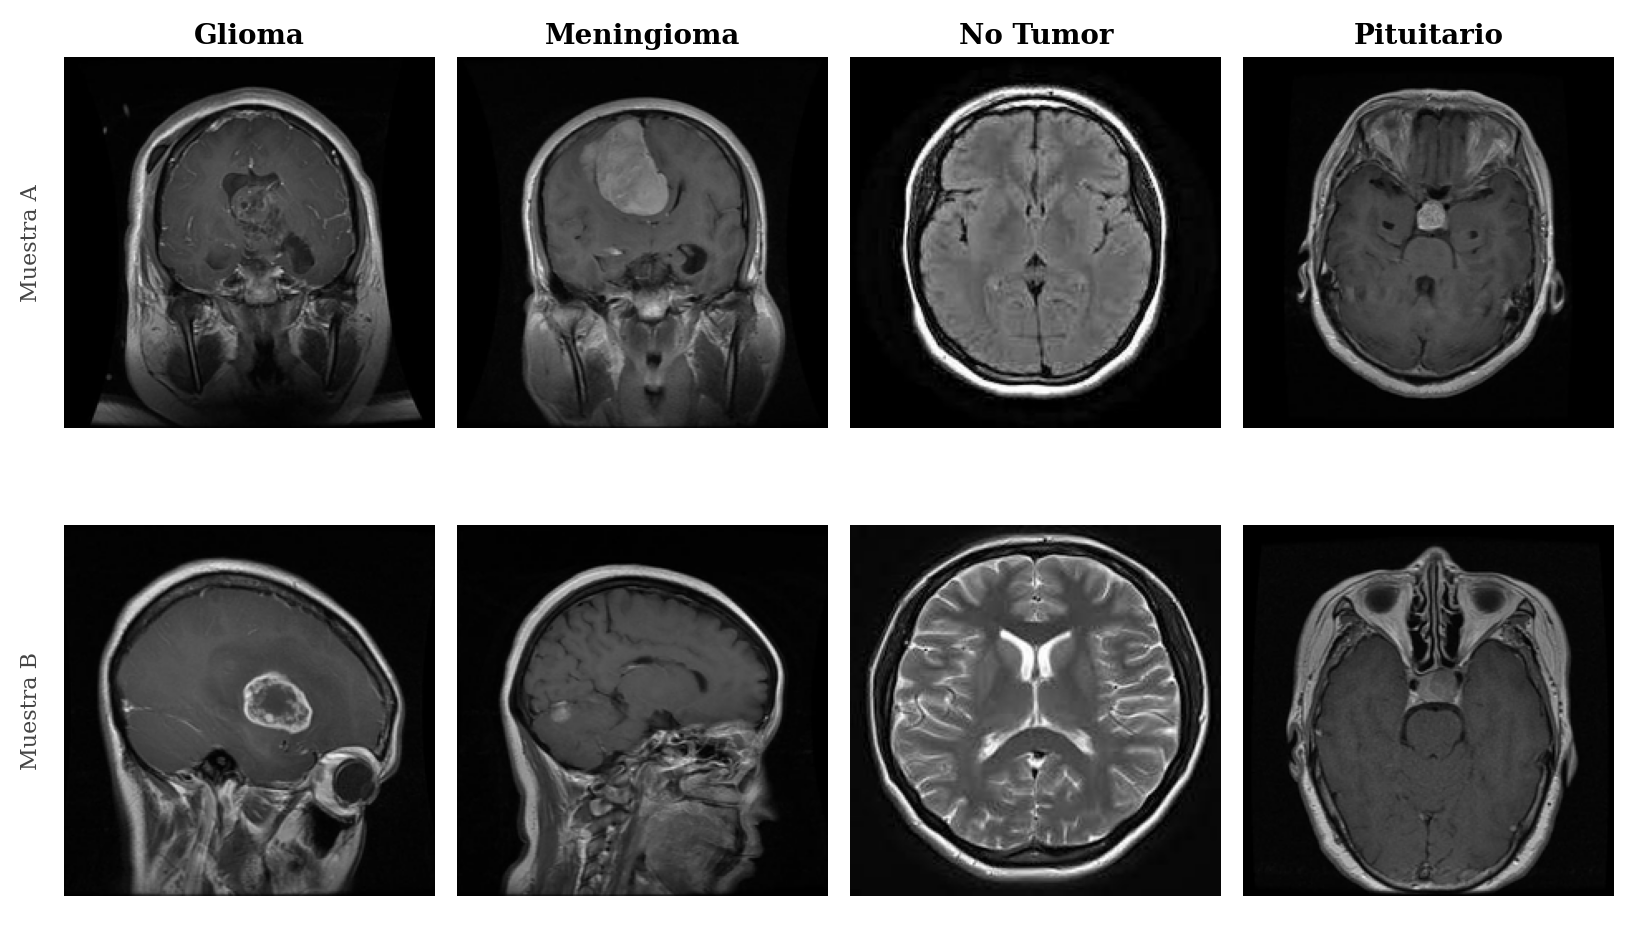
\includegraphics[width=\linewidth]{images/fig_brain_tumor_samples.png}
  \caption{Muestras representativas del dataset Brain Tumor MRI, ilustrando la variabilidad visual intra-clase e inter-clase entre las cuatro categorías diagnósticas.}
  \label{fig:fig_brain_tumor_samples}
  \vspace{0.2cm}
  \small Fuente: Kaggle Brain Tumor MRI Dataset \cite{msoud_nickparvar_2026}.
\end{figure}

\subsection{CIFAR-10}

CIFAR-10 se empleó como dataset de referencia estándar \cite{krizhevsky2009learning}. Contiene $60\,000$ imágenes de
$32 \times 32$ píxeles distribuidas en diez clases, con $50\,000$ imágenes de entrenamiento
y $10\,000$ de prueba. Todas las imágenes se redimensionaron a $224 \times 224$ para
mantener la misma resolución de entrada que en Brain Tumor MRI. El preprocesamiento incluyó
volteo horizontal aleatorio y normalización con las estadísticas propias del dataset. 
En test se aplicó únicamente redimensionamiento y normalización.


\begin{figure}[htbp]
  \centering
  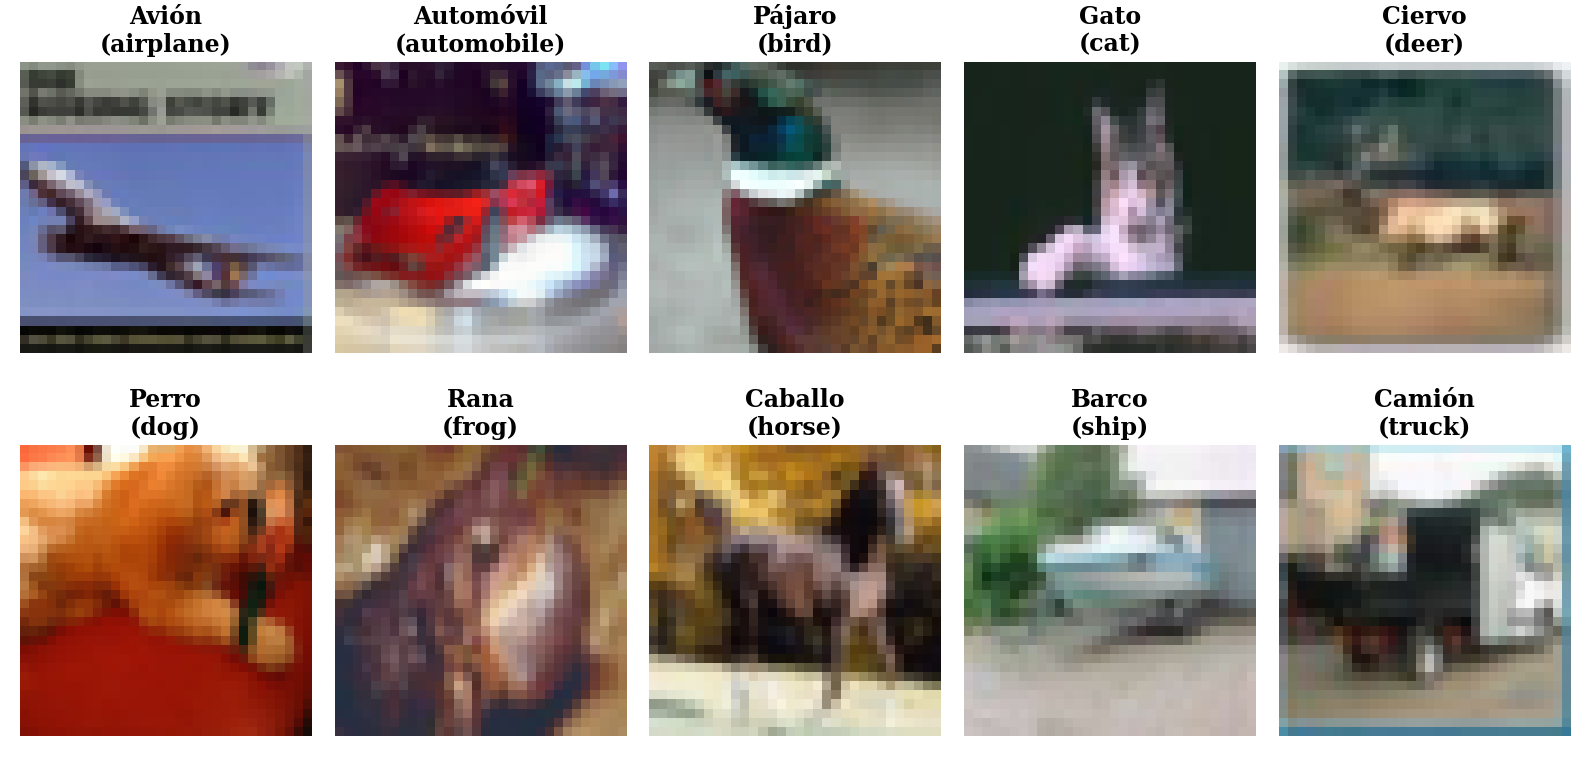
\includegraphics[width=\linewidth]{images/fig_cifar10_samples.png}
  \caption{Muestras representativas del dataset CIFAR-10 (una imagen por clase,
           resolución original $32\times32$ px). Las diez clases cubren objetos
           cotidianos de transporte, animales y vehículos.}
  \label{fig:fig_cifar10_samples}
  \vspace{0.2cm}
  \small Fuente: CIFAR-10 \cite{msoud_nickparvar_2026}.
\end{figure}



\subsection{Configuración del DataLoader}

En todos los experimentos se utilizó \texttt{DataLoader} con \texttt{batch\_size = 32},
\texttt{shuffle = True}, \texttt{num\_workers = 2} y \texttt{pin\_memory = True}. El
parámetro \texttt{drop\_last = True} fue obligatorio para los modelos con BatchNorm, ya que
un batch de tamaño unitario al final de una época local provoca una división por cero en el
cálculo de la varianza del batch.

% ============================================================
\section{Particionamiento Federado No-IID}
% ============================================================

\subsection{Estrategia Dirichlet}

La heterogeneidad estadística entre clientes se generó mediante particiones de Dirichlet
sobre las etiquetas de entrenamiento. Para $C$ clases y $K = 10$ clientes, se muestreó un
vector de proporciones $\mathbf{q}_k \sim \text{Dir}(\alpha \cdot \mathbf{1}_C)$ por clase y
se asignó a cada cliente $k$ la fracción $q_{k,c}$ de las muestras de la clase $c$. Cuando
algún cliente recibía menos de diez muestras de una clase asignada, se aplicó un paso de
redistribución para garantizar ese mínimo.

Se evaluaron cinco niveles de heterogeneidad: $\alpha \in \{1000, 1.0, 0.3, 0.1, 0.03\}$, 
siguiendo una configuración similar propuesta por \cite{jimenez2503thorough}.
El valor $\alpha = 1000$ produce una partición prácticamente IID; $\alpha = 0.03$ concentra
la mayoría de las muestras de cada clase en uno o dos clientes. La Tabla~\ref{tab:alpha_levels}
resume la correspondencia entre $\alpha$ y el nivel de heterogeneidad.

\begin{table}[H]
\centering
\caption{Niveles de heterogeneidad evaluados según el parámetro $\alpha$ de Dirichlet.}
\label{tab:alpha_levels}
\begin{tabular}{cll}
\hline
$\alpha$ & Nivel & Distancia de Hellinger aproximada \\
\hline
1000  & IID (línea base) & $\approx 0.00$ \\
1.0   & Baja             & $\approx 0.50$ \\
0.3   & Moderada         & $\approx 0.65$ \\
0.1   & Alta             & $\approx 0.80$ \\
0.03  & Extrema          & $\approx 0.90$ \\
\hline
\end{tabular}
\end{table}


\begin{figure}[htbp]
  \centering
  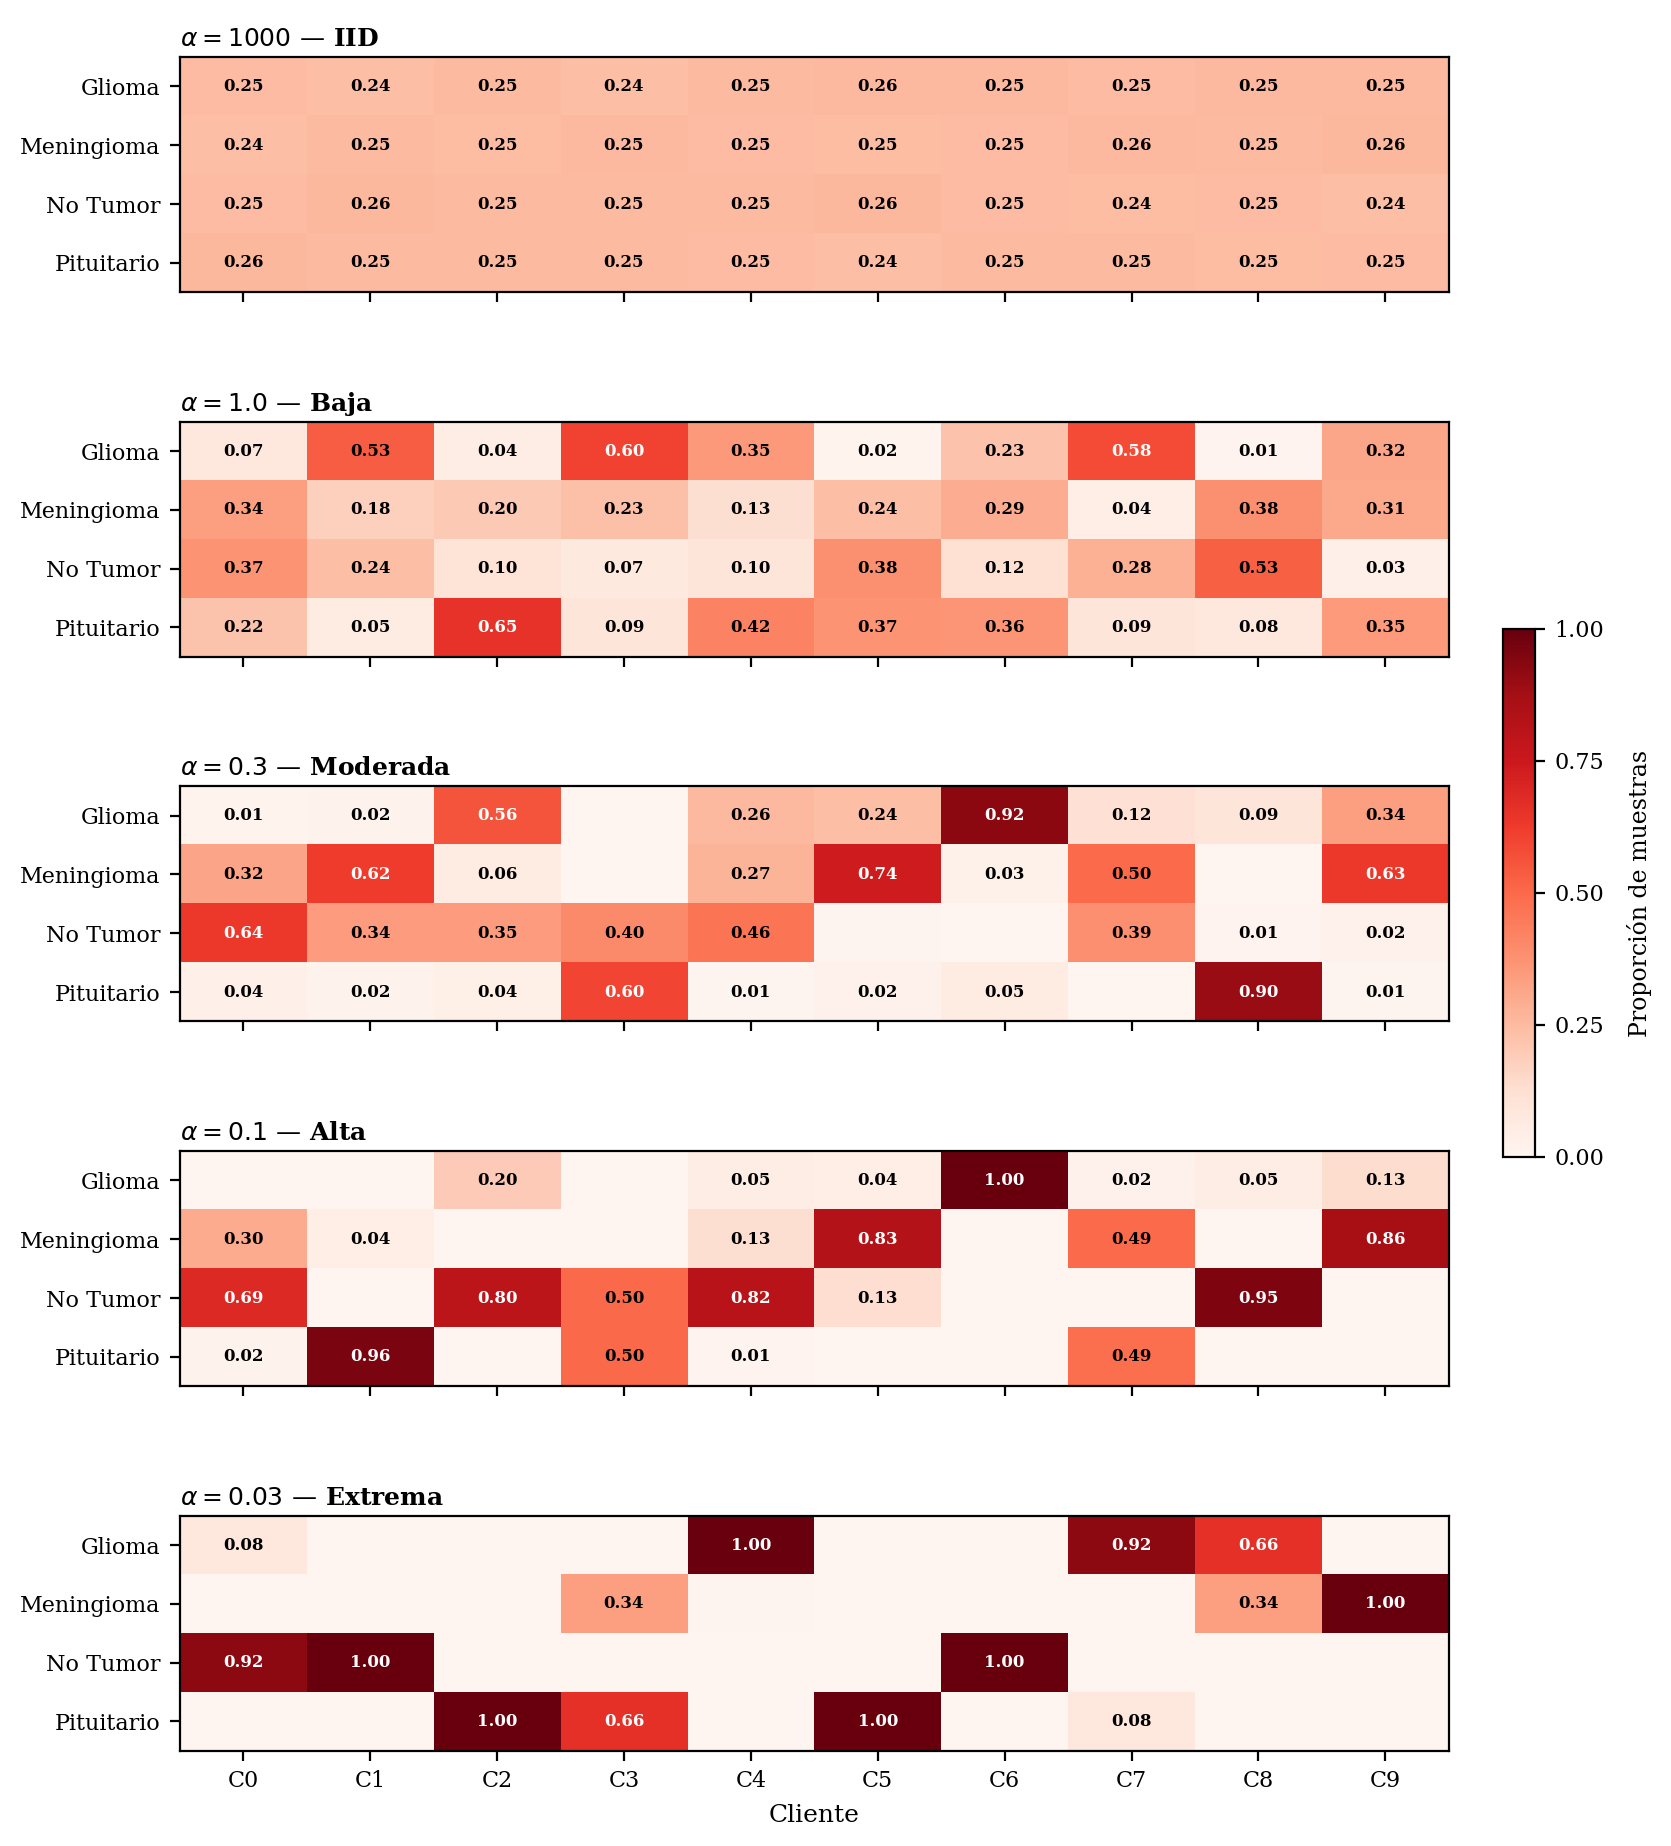
\includegraphics[width=\linewidth]{images/fig_dirichlet_partitions.png}
  \caption[Particiones Dirichlet — Brain Tumor MRI]{%
    Distribución de etiquetas por cliente bajo particiones
    Dirichlet para cinco niveles de heterogeneidad ($K=10$, semilla 42).
    Cada celda indica la proporción de muestras de esa clase asignadas al cliente.
    A medida que $\alpha$ decrece, la concentración por clase aumenta y la
    variabilidad inter-cliente se amplifica.}
  \label{fig:fig_dirichlet_partitions}

\end{figure}


\subsection{Reproducibilidad de las particiones}

Cada partición se generó con una semilla fija mediante \texttt{generate\_data.py} y se
almacenó en \path{data/{dataset}/partitions/alpha_{a}/seed_{seed}/}.
Cada directorio contiene \texttt{partition.pkl} con los índices por cliente y
\texttt{all\_stats.json} con la distribución de etiquetas, entropía y Distancia de Hellinger
por cliente. El uso de la misma semilla garantiza particiones idénticas entre modelos y
algoritmos, de modo que las diferencias observadas en el drift son atribuibles a la
arquitectura y no a variaciones en los datos.

El conjunto de prueba no se particionó: todos los clientes y el servidor evalúan sobre el
mismo test global, lo que permite comparar el rendimiento de generalización sin ambigüedad.

% ============================================================
\section{Modelos Evaluados}
% ============================================================

\subsection{Especificaciones de las arquitecturas}

Se evaluaron siete variantes de modelo pertenecientes a cuatro familias arquitectónicas.
La Tabla~\ref{tab:models} resume sus especificaciones principales. Todos los modelos se
inicializaron con pesos aleatorios para aislar el efecto
de la arquitectura sobre el drift sin confundir con representaciones preaprendidas. Esta
decisión implica una convergencia más lenta y una precisión final menor que con
preentrenamiento, en particular sobre Brain Tumor MRI (${\sim}7\,000$ imágenes); los
resultados deben interpretarse como medición del comportamiento de drift arquitectónico
bajo federación y no como benchmarks de clasificación absolutos.

\begin{table}[H]
\centering
\caption{Especificaciones de los siete modelos evaluados.}
\label{tab:models}
\resizebox{\textwidth}{!}{%
\begin{tabular}{llllll}
\hline
Modelo & Clave & Familia & Normalización & Dim. emb. & Bloques \\
\hline
EfficientNet-B1 (BN) & \texttt{efficient1}     & CNN & BatchNorm2d            & --- & 8 etapas \\
EfficientNet-B1 (GN) & \texttt{efficient1\_gn} & CNN & GroupNorm-32           & --- & 8 etapas \\
EfficientNet-B1 (LN) & \texttt{efficient1\_ln} & CNN & GroupNorm-1 ($\equiv$ LN) & --- & 8 etapas \\
ViT-Tiny             & \texttt{vit\_tiny}      & ViT & LayerNorm              & 192 & 12 bloques Transformer \\
Vim-Tiny             & \texttt{vim\_tiny}      & SSM & RMSNorm (fusionado)    & 192 & 12 bloques SSM \\
ViG-Tiny             & \texttt{vig\_tiny}      & GNN & BatchNorm2d            & 192 & 12 bloques Grapher \\
ResNet-9             & \texttt{res9}           & CNN & BatchNorm2d            & --- & 4 etapas + 2 res. \\
\hline
\end{tabular}}
\end{table}

\begin{center}
\textit{[FIGURA M5: Diagramas de bloque de las cuatro familias arquitectónicas evaluadas]}\\
\textit{Descripción: Cuatro paneles, uno por familia. (a) EfficientNet-B1: bloque MBConv con}
\textit{convolución depthwise + SE, con las capas de normalización indicadas en color.}
\textit{(b) ViT-Tiny: bloque Transformer con MHSA y MLP, LayerNorm en posición pre-norm.}
\textit{(c) Vim-Tiny: bloque SSM bidireccional con escaneo forward/backward y RMSNorm.}
\textit{(d) ViG-Tiny: bloque Grapher con construcción del grafo $k$-NN y propagación de mensajes.}
\textit{En cada panel se indica el número de bloques, la dimensión de embedding y la normalización.}
\textit{Propósito: mostrar en una sola figura las diferencias estructurales entre familias que}
\textit{determinan los distintos sesgos inductivos y perfiles de drift.}\\
\textit{Fuente: elaboración propia, basada en las referencias originales de cada arquitectura.}
\end{center}

\subsection{Ablación de normalización sobre EfficientNet-B1}

Las tres variantes de EfficientNet comparten exactamente el mismo sesgo inductivo
convolucional —bloques MBConv, módulos Squeeze-and-Excitation y jerarquía de
características— y difieren únicamente en la estrategia de normalización. La función
\texttt{replace\_batchnorm()} sustituyó recursivamente todos los módulos
\texttt{BatchNorm2d} por \texttt{GroupNorm(32)} o \texttt{GroupNorm(1)} $\equiv$
\texttt{LayerNorm} sobre la CNN base, preservando el número de parámetros aprendibles.
Esta ablación permite atribuir las diferencias de drift observadas entre variantes a la
normalización y no al mecanismo de extracción de características.

\subsection{Registro en FL-bench}

Como base de software para la experimentación se utilizó el repositorio
\textit{FL-bench} \cite{Tan_FL-bench}, un framework de
código abierto para la evaluación de algoritmos de aprendizaje federado. El repositorio
provee la infraestructura de comunicación cliente-servidor, la interfaz \texttt{DecoupledModel},
los algoritmos FedAvg y FedProx, y el pipeline de entrenamiento federado sobre el que se
construyeron todas las extensiones de este trabajo (registro de métricas de drift, cómputo
offline de CKA y scheduler del lado del servidor).

Todos los modelos se registraron en el diccionario \texttt{MODELS} de
\texttt{src/utils/models.py}, heredando de \texttt{DecoupledModel} y definiendo
\texttt{self.base} (extractor de características) y \texttt{self.classifier} (cabeza de
clasificación). ViG-Tiny se importa desde \texttt{Vision\_GNN/} mediante inyección de
\texttt{sys.path} en el momento de la construcción; el wrapper \texttt{\_ViGBase} sirve
únicamente para satisfacer la interfaz de \texttt{DecoupledModel}. Vim-Tiny requiere
\texttt{mamba\_ssm} con kernels CUDA fusionados; la importación está protegida por un
bloque \texttt{try/except} con mensaje de error informativo.

% ============================================================
\section{Protocolo de Aprendizaje Federado}
% ============================================================

\subsection{Configuración experimental}

La Tabla~\ref{tab:fl_config} resume los hiperparámetros del protocolo federado, comunes a
todos los experimentos. Se empleó una topología \textit{cross-silo} con $K = 10$ clientes
de participación completa en cada ronda, eliminando el ruido de muestreo del análisis de
drift. El número de rondas se fijó en $T = 50$ para observar tanto la dinámica temprana del
drift (rondas 1--10) como el comportamiento de convergencia tardía.

\begin{table}[H]
\centering
\caption{Hiperparámetros del protocolo federado.}
\label{tab:fl_config}
\begin{tabular}{ll}
\hline
Parámetro                        & Valor \\
\hline
Número de clientes ($K$)         & 10 \\
Participación por ronda          & 1.0 (100\%) \\
Rondas de comunicación ($T$)     & 50 \\
Épocas locales ($E$)             & 5 \\
Tamaño de batch ($B$)            & 32 \\
Optimizador                      & SGD (momentum $= 0.9$, wd $= 10^{-4}$) \\
Tasa de aprendizaje inicial      & 0.01 \\
Scheduler de LR                  & CosineAnnealingLR (lado servidor) \\
$\mu$ FedProx                    & 0.01 \\
Semillas                         & 42, 123, 456 \\
\hline
\end{tabular}
\end{table}

El scheduler de tasa de aprendizaje se implementó del lado del servidor para garantizar
que todos los clientes inicien cada ronda con el mismo LR globalmente decaído. FL-bench
avanza el scheduler una vez por época local, lo que produciría $E = 5$ veces más pasos que
los deseados. El servidor calcula el LR coseno correspondiente a la ronda $t$ e inyecta el
valor en \texttt{args.optimizer.lr}; los clientes construyen su optimizador con ese valor
al inicio de cada ronda (\texttt{reset\_optimizer\_on\_global\_epoch: true}).

\subsection{Ciclo de una ronda de comunicación}

El protocolo de cada ronda $t$ siguió los siguientes pasos:

\begin{enumerate}
  \item El servidor difunde el modelo global $\boldsymbol{\theta}^{(t-1)}$ a los $K$
    clientes.
  \item Cada cliente $k$ ejecuta $E$ épocas de SGD local sobre $\mathcal{D}_k$, obteniendo
    $\boldsymbol{\theta}_k^{(t)}$.
  \item \textbf{Antes de la agregación}: el servidor registra el drift $L_2$ por grupo de
    capas y la similitud coseno inter-cliente para cada par de clientes.
  \item El servidor agrega: $\boldsymbol{\theta}^{(t)} = \sum_k (n_k/n)\,
    \boldsymbol{\theta}_k^{(t)}$.
  \item \textbf{Después de la agregación}: el servidor evalúa accuracy y F1 sobre el test
    global y registra equidad inter-cliente.
  \item En las rondas de checkpoint programadas $\{1, 2, 5, 10, 20, 30, 40, 50\}$, se
    guardan el estado del modelo global pre-agregación y los estados de todos los clientes
    post-entrenamiento, para el cómputo offline de CKA.
\end{enumerate}

\begin{center}
\textit{[FIGURA M6: Diagrama de flujo de una ronda de comunicación federada]}\\
\textit{Descripción: Diagrama vertical con cinco bloques secuenciales: (1) broadcast del}
\textit{modelo global a los 10 clientes; (2) entrenamiento local paralelo en cada cliente}
\textit{($E=5$ épocas de SGD); (3) registro de métricas de drift ANTES de la agregación;}
\textit{(4) agregación FedAvg/FedProx en el servidor; (5) evaluación global y guardado de}
\textit{checkpoint condicional. Las ramas de FedAvg y FedProx se distinguen en el bloque (4).}
\textit{Propósito: mostrar con precisión el orden de las operaciones en cada ronda, en especial}
\textit{la posición del registro de métricas respecto a la agregación.}\\
\textit{Fuente: elaboración propia.}
\end{center}

% ============================================================
\section{Taxonomía de Capas para el Análisis de Drift}
% ============================================================

Para hacer comparables las métricas de drift entre familias arquitectónicas con estructuras
internas heterogéneas, los parámetros de cada modelo se clasificaron en tres grupos
funcionales mediante la función \texttt{classify\_layer(name, module)} implementada en
\texttt{src/utils/drift\_metrics.py}:

\begin{itemize}
  \item \textbf{norm}: parámetros aprendibles ($\gamma$, $\beta$) de las capas de
    normalización (BatchNorm2d, GroupNorm, LayerNorm, RMSNorm).
  \item \textbf{feature}: pesos de las capas de extracción de características
    (Conv2d, proyecciones lineales internas), excluida la cabeza clasificadora.
  \item \textbf{head}: parámetros de la capa clasificadora final.
\end{itemize}

Los buffers de BatchNorm (\texttt{running\_mean}, \texttt{running\_var},
\texttt{num\_batches\_tracked}) se excluyen del cómputo, ya que no participan en la
agregación FedAvg. Los módulos de activación y pooling se clasifican como \texttt{other}
y quedan fuera de todas las métricas de drift.

La Tabla~\ref{tab:layer_taxonomy} especifica la correspondencia entre esta taxonomía y los
módulos concretos de cada arquitectura.

\begin{table}[H]
\centering
\caption{Taxonomía de capas por arquitectura.}
\label{tab:layer_taxonomy}

\begin{tabularx}{\textwidth}{l l X l}
\hline
Arquitectura & \textbf{norm} & \textbf{feature} & \textbf{head} \\
\hline
EfficientNet-B1 & BN / GN / LN layers & Bloques MBConv (Conv2d, SE) & FC clasificador \\
ViT-Tiny & LayerNorm layers & Atención (Q, K, V) + MLP & Proj. sobre [CLS] \\
Vim-Tiny & RMSNorm layers & Proyecciones SSM (B, C, $\Delta$) & FC clasificador \\
ViG-Tiny & BN layers & Bloques Grapher + FFN & FC clasificador \\
ResNet-9 & BN layers & Conv2d, bloques residuales & FC clasificador \\
\hline
\end{tabularx}
\end{table}

% ============================================================
\section{Métricas de Drift Paramétrico}
% ============================================================

\subsection{\texorpdfstring{Divergencia de pesos $L_2$}{Divergencia de pesos L2} por grupo de capas}

Para cada cliente $k$, grupo de capas $\ell \in \{\text{norm, feature, head}\}$ y ronda
$t$, se calcularon dos variantes complementarias de drift:

\textbf{Drift crudo} (escala-dependiente):
\begin{equation}
  \text{drift\_raw}_k^{(\ell)}(t) =
  \left\|\boldsymbol{\theta}_k^{(\ell)}(t) - \boldsymbol{\theta}_{\text{global}}^{(\ell)}
  (t-1)\right\|_2.
  \label{eq:drift_raw}
\end{equation}

\textbf{Drift normalizado RMS} (escala-independiente):
\begin{equation}
  \text{drift\_norm}_k^{(\ell)}(t) =
  \frac{\text{drift\_raw}_k^{(\ell)}(t)}{\sqrt{N^{(\ell)}}},
  \label{eq:drift_norm}
\end{equation}

donde $N^{(\ell)}$ es el número total de parámetros escalares en el grupo $\ell$. Esta
normalización convierte el valor en el drift RMS por parámetro, permitiendo comparaciones
directas entre grupos de tamaños muy distintos y entre arquitecturas. Todas las comparaciones
cross-arquitectura de este trabajo emplean \texttt{drift\_norm}; el drift crudo se retiene
para verificar que el término proximal de FedProx acota la magnitud absoluta esperada.

Para cada ronda se reportan la media y desviación estándar del drift normalizado sobre los
$K = 10$ clientes, por grupo de capas.

\subsection{Alineación de gradientes inter-cliente}

La similitud coseno pairwise por grupo de capas y ronda cuantifica si las actualizaciones
de distintos clientes son constructivas o destructivas al ser promediadas:

\begin{equation}
  \text{alignment}^{(\ell)}(t) = \frac{1}{K(K-1)}
  \sum_{i=1}^{K} \sum_{j \neq i}
  \frac{\mathbf{g}_i^{(\ell)}(t) \cdot \mathbf{g}_j^{(\ell)}(t)}
  {\left\|\mathbf{g}_i^{(\ell)}(t)\right\|_2 \left\|\mathbf{g}_j^{(\ell)}(t)\right\|_2},
  \label{eq:cosine}
\end{equation}

donde $\mathbf{g}_k^{(\ell)}(t) = \boldsymbol{\theta}_{\text{global}}^{(\ell)}(t-1) -
\boldsymbol{\theta}_k^{(\ell)}(t)$ es el pseudo-gradiente del cliente $k$ en el grupo
$\ell$. Valores positivos indican actualizaciones constructivas; valores negativos,
interferencia destructiva.

Ambas métricas se registran \textit{antes} de la agregación en cada ronda, en
\texttt{DriftFedAvgServer.aggregate\_client\_updates()} y su análogo para FedProx, y se
almacenan en \texttt{drift\_metrics.csv}.

\begin{center}
\textit{[FIGURA M7: Pipeline de registro de métricas paramétricas durante el entrenamiento]}\\
\textit{Descripción: Diagrama de flujo detallado del interior del bloque de agregación de la}
\textit{Figura M6. Muestra la secuencia: (1) recepción de los $K$ state dicts de clientes;}
\textit{(2) cálculo de drift raw y norm para cada cliente y grupo de capas; (3) cálculo de}
\textit{similitud coseno pairwise para cada grupo; (4) escritura en \texttt{drift\_metrics.csv};}
\textit{(5) guardado de checkpoints condicional (rondas programadas); (6) promedio FedAvg/FedProx.}
\textit{Propósito: documentar el orden exacto de las operaciones y el punto de captura de datos,}
\textit{garantizando la trazabilidad del momento de medición respecto a la agregación.}\\
\textit{Fuente: elaboración propia.}
\end{center}

% ============================================================
\section{Análisis de Representaciones mediante CKA}
% ============================================================

\subsection{Arquitectura del pipeline offline}

El cómputo de CKA se desacopló completamente del entrenamiento para eliminar la presión sobre
la memoria GPU. El flujo se divide en dos etapas diferenciadas:

\textbf{Durante el entrenamiento} (\texttt{CKADriftFedAvgServer}): en las rondas programadas
$\{1, 2, 5, 10, 20, 30, 40, 50\}$, el servidor guarda en disco el estado del modelo global
pre-agregación (\texttt{global.pt}) y el estado de cada cliente post-entrenamiento local
(\texttt{client\_k.pt}), junto con los metadatos del experimento (\texttt{run\_metadata.json}).
No se realizan forward passes ni cálculos de activaciones durante el entrenamiento.

\textbf{Después del entrenamiento} (scripts offline en \texttt{scripts/}):
\begin{itemize}
  \item \texttt{compute\_cka\_offline.py}: calcula el CKA global-vs-cliente para cada ronda
    programada y guarda los resultados en \texttt{cka\_metrics.csv} y matrices completas en
    \texttt{cka\_matrices/*.npz}.
  \item \texttt{compute\_client\_cka\_offline.py}: calcula el CKA pairwise entre todos los
    pares de clientes y guarda en \texttt{client\_cka\_metrics.csv}.
\end{itemize}

\begin{center}
\textit{[FIGURA M8: Pipeline CKA — fases durante y después del entrenamiento]}\\
\textit{Descripción: Diagrama de dos columnas. Columna izquierda (durante entrenamiento):}
\textit{el servidor entrena T=50 rondas; en las rondas programadas $\{1,2,5,10,20,30,40,50\}$}
\textit{guarda checkpoints (global.pt + client\_k.pt) sin interrumpir el entrenamiento.}
\textit{Columna derecha (post-entrenamiento): los scripts offline leen los checkpoints,}
\textit{ejecutan forward passes en CPU, calculan CKA y escriben los CSV de resultados.}
\textit{Propósito: documentar la separación entre el entrenamiento y el análisis representacional,}
\textit{justificando la decisión de diseño que evita presión sobre la memoria GPU.}\\
\textit{Fuente: elaboración propia.}
\end{center}

\subsection{Mapa de capas por arquitectura}

Los puntos de hook para la recolección de activaciones se determinaron a partir de los
nombres exactos de los módulos expuestos por \texttt{named\_modules()}, ya que la lógica de
registro de hooks se implementó con coincidencia exacta de nombre. La
Tabla~\ref{tab:cka_layers} resume el número de capas monitoreadas por modelo.

\begin{table}[H]
\centering
\caption{Capas monitoreadas para CKA por arquitectura.}
\label{tab:cka_layers}

\begin{tabularx}{\textwidth}{l c X}
\hline
Modelo & $N_{\text{capas}}$ & Observaciones \\
\hline

EfficientNet-B1 (×3) & 10 &
\texttt{base.features.0--8} + \texttt{classifier} \\

ViT-Tiny & 15 &
\texttt{base.patch\_embed} + \texttt{base.blocks.0--11} +
\texttt{base.norm} + \texttt{classifier} \\

Vim-Tiny & 14 &
\texttt{base.patch\_embed} + \texttt{base.layers.0--11.mixer} +
\texttt{classifier} \newline
(capas norm excluidas: kernel CUDA fusionado no dispara hook) \\

ViG-Tiny & 14 &
\texttt{\_vig\_stem} + \texttt{\_vig\_blocks.0--11} +
\texttt{classifier} \newline
(módulos en raíz del objeto, no bajo \texttt{self.base}) \\

ResNet-9 & 9 &
\texttt{base.2}, \texttt{base.6}, \texttt{base.7},
\texttt{base.11}, \texttt{base.15--18} +
\texttt{classifier} \\

\hline
\end{tabularx}
\end{table}

\subsection{Análisis CKA global-vs-cliente}

Para cada ronda programada $t$ y cliente $k$, se cargaron \texttt{global.pt} y
\texttt{client\_k.pt}, se hicieron pasar $N_{\text{probe}} \leq 512$ muestras por ambos
modelos en CPU y se calculó el CKA diagonal entre las activaciones de capas homólogas:

\begin{equation}
  \text{CKA\_gc}_{k}^{(\ell)}(t) = \text{CKA}\!\left(
    \mathbf{X}_{k}^{(\ell)}(t),\; \mathbf{X}_{\text{global}}^{(\ell)}(t)
  \right),
  \label{eq:cka_gc}
\end{equation}

donde $\mathbf{X}_{k}^{(\ell)}$ y $\mathbf{X}_{\text{global}}^{(\ell)}$ son las matrices de
activación de la capa $\ell$ evaluadas sobre el mismo conjunto de muestras de referencia.
Un valor cercano a 1 indica que el cliente conserva representaciones funcionalmente alineadas
con el modelo global; un valor cercano a 0 indica divergencia representacional.

\subsection{Análisis CKA pairwise inter-cliente}

Para cada par de clientes $(i, j)$ y ronda programada $t$, se calculó el CKA entre sus
activaciones sobre las mismas muestras de referencia. Este análisis complementa el
global-vs-cliente al cuantificar si distintos clientes están aprendiendo representaciones
similares entre sí, independientemente del modelo global.

\subsection{Gestión de memoria}

Los forward passes de CKA se ejecutaron en CPU. Las activaciones espaciales (tensores 4D)
se redujeron a 2D mediante pooling global antes del almacenamiento en RAM. Se limitó el
número de muestras de sondeo a 512 filas por capa, lo que es suficiente para estimados CKA
estables según \cite{DBLP:journals/corr/abs-1905-00414}. Los parámetros
\texttt{probe\_batches = 20} y \texttt{probe\_batch\_size = 16} se registraron en
\texttt{run\_metadata.json} para garantizar la reproducibilidad del análisis offline.

% ============================================================
\section{Métricas de Evaluación del Rendimiento}
% ============================================================

\subsection{Métricas de clasificación}

Tras cada ronda de comunicación se evaluó el modelo global sobre el test global y se
calcularon accuracy, F1-score macro, precision macro y recall macro. El F1-score macro es la
métrica primaria para Brain Tumor MRI por su robustez ante variaciones en la distribución
de clases bajo particiones Dirichlet; la
accuracy es la métrica primaria para CIFAR-10.

\subsection{Velocidad de convergencia}

La convergencia se definió como la primera ronda $t$ en que la accuracy global cruza el
umbral establecido —70\,\% para CIFAR-10 y 80\,\% para Brain Tumor MRI— y permanece por
encima durante cinco rondas consecutivas. Los modelos que no alcanzaron la convergencia en
$T = 50$ rondas se registraron con \texttt{convergence\_round = -1}.

\subsection{Equidad inter-cliente}

La equidad se midió como la brecha de accuracy entre el cliente con mayor y menor rendimiento
al final del entrenamiento (\textit{fairness gap}). Como indicador secundario se reportó la
desviación estándar de accuracy entre los diez clientes.

\subsection{Agregación estadística}

Todos los resultados se reportan como $\mu \pm \sigma$ sobre las tres semillas $\{42, 123,
456\}$. Las ejecuciones con desviación estándar de accuracy superior a $0.03$ se marcaron
como alta varianza para inspección adicional. Para las comparaciones clave entre
arquitecturas se aplicó la prueba de Wilcoxon signed-rank (no paramétrica, $\alpha = 0.05$).
Dado el tamaño de muestra reducido ($n = 3$ semillas), los $p$-values se reportan como
indicativos y no definitivos.

% ============================================================
\section{Estudios de Ablación}
% ============================================================

Se diseñaron cinco estudios de ablación para aislar los factores de mayor interés. Los tres
primeros son primarios y forman parte del análisis principal; los dos últimos son secundarios.

\textbf{Ablación 1 — Normalización.} Se compararon EfficientNet-B1 en sus tres variantes (BN,
GN-32, LN) bajo configuración FL idéntica. El gap en drift, accuracy y CKA entre variantes
cuantifica la contribución específica de BatchNorm frente al sesgo inductivo convolucional.

\textbf{Ablación 2 — Heterogeneidad.} Para cada modelo se trazó la curva de accuracy vs.\
$\alpha$ sobre ambos datasets. El objetivo es identificar el valor crítico de $\alpha$ a
partir del cual el rendimiento de cada familia arquitectónica degrada de forma no lineal.

\textbf{Ablación 3 — Algoritmo federado.} Se compararon FedAvg y FedProx para cada
combinación modelo × dataset × $\alpha$, reportando las diferencias $\Delta_{\text{acc}}$,
$\Delta_{\text{drift}}$ y $\Delta_{\text{CKA}}$. La hipótesis es que FedProx beneficia
proporcionalmente más a las arquitecturas con mayor drift (BN-based).

\textbf{Ablación 4 — Intra-familia por normalización.} Se compararon los perfiles de drift L2
y CKA de los modelos con BatchNorm (EfficientNet-B1 BN, ViG-Tiny, ResNet-9) frente a los
modelos con normalización por muestra (ViT-Tiny, Vim-Tiny), independientemente de la familia.
Esta comparación separa el efecto de la normalización del efecto del sesgo inductivo.

\textbf{Ablación 5 — Épocas locales.} Se evaluaron $E \in \{1, 5, 10\}$ para una única
celda experimental ($\alpha = 0.1$, Brain Tumor MRI, FedAvg, semilla 42), con el objetivo de
verificar que el número de épocas locales amplifica el drift de forma diferenciada según
arquitectura.

% ============================================================
\section{Procedimiento Experimental}
% ============================================================

\begin{center}
\textit{[FIGURA M9: Diagrama general del procedimiento experimental]}\\
\textit{Descripción: Diagrama de flujo horizontal con nueve bloques secuenciales que}
\textit{representan las fases del experimento: (1) Configuración del entorno; (2) Preparación}
\textit{de datos y particionamiento; (3) Implementación de modelos; (4) Implementación de}
\textit{métricas de drift; (5) Implementación del pipeline CKA; (6) Ejecución de los 210 runs;}
\textit{(7) Verificación de integridad (50 filas por CSV, sanity check); (8) Análisis CKA}
\textit{offline; (9) Visualización y análisis estadístico. Las fases completadas se indican con}
\textit{una marca de verificación; las pendientes, con un reloj. Este diagrama refleja el estado}
\textit{real de avance al momento de la redacción.}\\
\textit{Fuente: elaboración propia.}
\end{center}

La ejecución experimental se organizó en nueve fases. Las fases 1 a 5 corresponden a la
preparación del entorno, la ingesta de datos, la implementación de modelos y la
instrumentación de métricas. La fase 6 ejecutó los 210 runs primarios: 7 modelos × 5 valores
de $\alpha$ × 3 semillas × 2 algoritmos sobre Brain Tumor MRI, con ejecuciones paralelas en
CIFAR-10 como referencia. La fase 7 verificó la integridad de los resultados mediante
\texttt{sanity\_check.py}, que detecta ejecuciones con accuracy final $< 0.1$, drift nulo o
alta varianza. Las fases 8 y 9 ejecutaron el análisis CKA offline y la generación de figuras.

La estructura de directorios de salida siguió el esquema:
\begin{center}
    \path{logs/runs/{dataset}_alpha{a}_{model}_{method}_seed{seed}/}
\end{center}

Cada directorio contiene: \texttt{drift\_metrics.csv} (50 filas, una por ronda),
\texttt{metrics.csv} (salida estándar de FL-bench), \texttt{main.log},
\texttt{events.out.tfevents.*} (TensorBoard), el subdirectorio \texttt{checkpoints/} con
los estados del modelo por ronda programada, y los ficheros CKA generados offline.

% ============================================================
\section{Infraestructura Tecnológica}
% ============================================================

\subsection{Hardware}

\textit{[COMPLETAR con: modelo de CPU, GPU (nombre, VRAM en GB), memoria RAM del sistema.]}

\subsection{Software}

\begin{table}[H]
\centering
\caption{Entorno de software utilizado.}
\label{tab:software}
\begin{tabular}{ll}
\hline
Componente              & Versión \\
\hline
Python                  & 3.11 \\
PyTorch                 & 2.6.0 \\
CUDA                    & \textit{[COMPLETAR]} \\
torchvision             & 0.21.0 \\
timm                    & 1.0.15 \\
vision-mamba / mamba\_ssm & 0.1.0 \\
scikit-learn            & 1.6.1 \\
numpy                   & 1.26.4 \\
pandas                  & 2.2.3 \\
matplotlib / seaborn    & 3.10.1 / 0.13.2 \\
TensorBoard             & 2.17.1 \\
\hline
\end{tabular}
\end{table}

La reproducibilidad del entorno se garantizó mediante \texttt{requirements\_locked.txt}
(salida de \texttt{pip freeze}) y \texttt{environment.txt} (versiones de CUDA, PyTorch y
especificaciones de GPU obtenidas mediante \texttt{nvidia-smi}), ambos archivos versionados
en el repositorio.
